\title{\pkg{eurostat}: Eurostat Open Data R Tools}
\author{Leo Lahti, Janne Huovari, Markus Kainu, Przemyslaw Biecek}

\maketitle

%An abstract of less than 150 words.
\abstract{Governmental institutions have started to release increasing amount of
their data resources for the public as open data in the recent
years. This is opening novel opportunities for research and citizen
science. The eurostat R package provides a suite of tools to access open data from Eurostat, including functions to search, download, and manipulate these data sets in an automated and reproducible manner. The online documentation provides further examples on how to visualize, summarize and interpret these spatio-temporal data sets. The package builds on and extends the preceding SmarterPoland and statfi packages and has been extensively tested by the user community. This package contributes to the growing ecosystem of R packages that provide generic tools for reproducible computational research in social science and humanities.}

Efficient tools to access and analyse data collections from the public
domain can greatly benefit reproducible research \citep{Gandrud13,
Boettiger2015}. When the data is available, the complete analytical
workflow spanning from raw data to the final publication can be made
available. Standardization and automatization of common data analysis
tasks via dedicated software packages can help to automate the
analysis workflow, thus greatly facilitate reproducibility and code
sharing and making data analysis more transparent and efficient.

Here, we introduce the eurostat R package that implements R tools to
access open data from
Eurostat \footnote{\url{http://ec.europa.eu/eurostat}}. Eurostat
provides a rich collection of demographic and economic data through
its open data portal. The portal currently includes ... data sets on
... between years ...

Despite many efforts to this direction, a dedicated R package for
eurostat open data has been missing. Our work extends our earlier CRAN
packages statfi \citep{statfi} and smarterpoland
\citep{smarterpoland}. Compared to this earlier work, we have now
implemented an expanded set of tools specifically focusing on the
eurostat data collection. The eurostat R package hence brings together
earlier, independent efforts by the package developers. It has been
actively developed by several contributors and based on the community
feedback in Github, with its first CRAN release in 2014. We are now
reporting the first mature version of the package that has been
improved and tested by multiple users, and includes features like
cache, handling dates, and using the tidy data
principles \citep{wickham2014}, with the help of the tidyr R
package \citep{tidyr}. The package or its predecessors have been
applied in several case studies by us and independent users including
Financial
Times\footnote{http://blog.revolutionanalytics.com/2015/04/financial-times-tracks-unemployment-with-r.html}.

The datamart \citep{datamart} and the quandl
\citep{quandl} R packages provide generic tools that can be used to access
certain versions of eurostat data. In contrast to these generic
database packages, our the eurostat package provides functionality
that is particularly tailored for this data collection. There is also
a development version for R package
\pkg{reurostat}\footnote{https://github.com/Tungurahua/reurostat} but this
does not seem to be actively maintained. The package
depends on or imports the following external R packages:
\CRANpkg{devtools} \citep{devtools}, \CRANpkg{dplyr} \citep{dplyr},
\CRANpkg{knitr} \citep{knitr}, \CRANpkg{ggplot2} \citep{ggplot2},
\CRANpkg{mapproj} \citep{mapproj}, \CRANpkg{plotrix} \citep{plotrix},
\CRANpkg{reshape2} \citep{reshape2}, \CRANpkg{rmarkdown}
\citep{rmarkdown}, \CRANpkg{stringi} \citep{stringi},
\CRANpkg{testthat} \citep{testthat}, and \CRANpkg{tidyr}
\citep{tidyr}. The eurostat R package is
part of the rOpenGov project
\citep{Lahti13icml}, which provides reproducible research tools for
computational social science and digital humanities.


The package provides tools to search and retrieve data from the
Eurostat open data portal, to convert identifiers in human-readable
formats and to select, modify and visualize the data. In this
manuscript, we provide a brief overview of the core functionality in
the current CRAN release version (1.2.1). For further examples, see
the package
vignette\footnote{https://github.com/rOpenGov/eurostat/vignette/eurostat\_tutorial.Rmd}.



\section{Search and download commands}

To install the CRAN release version, type in R:

\code{
install.packages("eurostat")
}

The complete table of contents of the database can be downloaded in R
with the function \code{get\_eurostat\_toc()} [HERE LINK TO EUROSTAT
PAGE WHERE THE DATA CAN BE BROWSED ONLINE]. The
function \code{search\_eurostat()} can be used to make a more focused
search over the table of contents. To retrieve data sets for
'disposable income', for instance, use:

\begin{example}
library(eurostat)
income <- search_eurostat("disposable income", type = "dataset")
\end{example}


The queried data type is specified in the above example with
the \code{type} argument. The options for this argument
include \dfn{'table'}, \dfn{'dataset'} or \dfn{'folder'}, referring to
different levels of hierarchy in the data organization: a table
resides in dataset, and the datasets are stored in a
folder. The \code{type} argument limits the search on a selected data
set type. Values from the code column list identifiers for specific
data sets. These can be used in subsequent download
commands. Alternatively, the dataset identifier codes can also be
browsed at the Eurostat
website\footnote{http://ec.europa.eu/eurostat/data/database}; check
the codes in the Data Navigation Tree listed after each dataset (in
parentheses).

To retrieve the data set with a particular identifier (tsdtr210, for
instance), use

\code{
dat <- get\_eurostat(id = 'tsdtr210', time\_format = "num")
}

Since the original data is annual in this example, we have selected a
numeric time variable as this is more convient for annual time series
than the default date format. The function call returns a table on
passenger transport statistics in various countries. The first lines
of the output are shown in Table~\ref{tab:getdatatable}.

\begin{table}[ht]
\centering
\begin{tabular}{rlllrr}
\toprule
  \hline
 & unit & vehicle & geo & time & values \\ 
  \hline
  1 & PC & BUS\_TOT & AT & 1990.00 & 11.00 \\ 
  2 & PC & BUS\_TOT & BE & 1990.00 & 10.60 \\ 
  3 & PC & BUS\_TOT & BG & 1990.00 &  \\ 
  4 & PC & BUS\_TOT & CH & 1990.00 & 3.70 \\ 
  5 & PC & BUS\_TOT & CY & 1990.00 &  \\ 
  6 & PC & BUS\_TOT & CZ & 1990.00 &  \\ 
   \hline
\bottomrule   
\end{tabular}
\caption{First lines of output from the \code{get\_eurostat} function for the data set with the identifier 'tsdtr210'.}
\label{tab:getdatatable}
\end{table}

Multidimensional data sets can be also visualized as triangular maps
(Figure~\ref{fig:plotrix}) based on
the \CRANpkg{plotrix} \citep{plotrix} package.


\begin{figure}
\setkeys{Gin}{width=0.5\textwidth}
\begin{center}
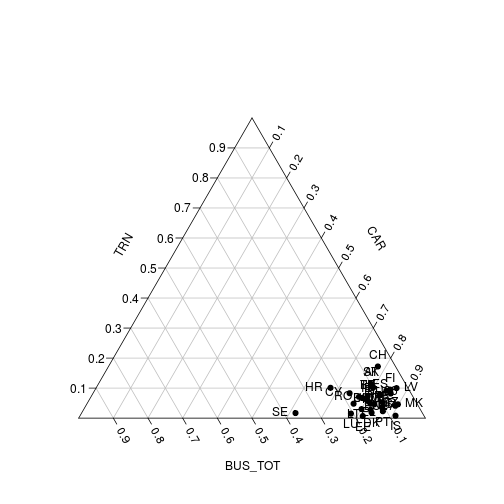
\includegraphics{2015-manu-search2-1}
\end{center}
\caption{Passenger transport data visualization on a triangular map.}
\label{fig:plotrix}
\end{figure}


To improve the interpretability of the output, the eurostat variable
identifiers could be further replaced with human-readable labels based
on definitions from Eurostat dictionaries with
the \code{label\_eurostat()} function. The data is provided in the
standard data.frame format, so that all standard tools for data
subsetting and reshaping are supported.


\section{Usage examples}

Eurostat provides a number of data sets of demographics and
economics. We can look, for instance, at the distribution of body-mass
index (BMI) indicating differences in obesity between different age
groups as visualized in Figure~\ref{fig:bmi}, or observe a decreasing
trend of road accidents in many countries over time
(Figure~\ref{fig:roadaccidents})\footnote{http://pbiecek.github.io/archivist/justGetIT.html}.


\begin{figure}
\setkeys{Gin}{width=0.5\textwidth}
\begin{center}
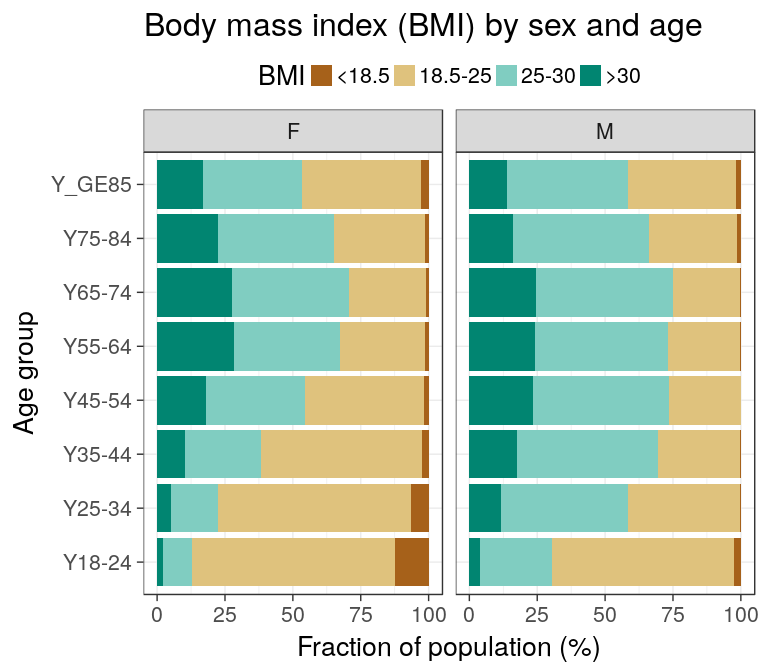
\includegraphics{2015-manu-bmi-1}
\end{center}
\caption{The body-mass index in different age groups based on Eurostat open data.}
\label{fig:bmi}
\end{figure}


\begin{figure}
\setkeys{Gin}{width=0.5\textwidth}
\begin{center}
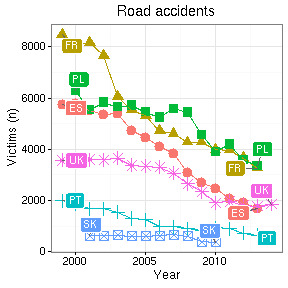
\includegraphics{2015-manu-roadacc-1}
\end{center}
\caption{Time series of the number of people killed in road accidents.}
\label{fig:roadaccidents}
\end{figure}





\section{Geospatial information}

Spatial information is conveniently visualized on a map. Most
indicators are of country/year-type, although sometimes data is
available also at more detailed levels of regional breakdown. Our
related blog
post\footnote{http://ropengov.github.io/r/2015/05/01/eurostat-package-examples}
provides a detailed description on geospatial data visualization,
looking at disposable income of private households (eurostat id
tgs00026\footnote{http://ec.europa.eu/eurostat/en/web/products-datasets/-/TGS00026})
at the NUTS2
regions\footnote{http://en.wikipedia.org/wiki/Nomenclature\_of\_Territorial\_Units\_for\_Statistics}
(Figure~\ref{fig:mapexample}).

In addition to downloading and manipulating data from Eurostat, we
demonstrate how to access and use the Eurostat geospatial data
(shapefiles) on administrative statistical
units\footnote{http://ec.europa.eu/eurostat/web/gisco/geodata/reference-data/administrative-units-statistical-units}
to visualize the income statistics on the European map. The example
demonstrates how the Eurostat data sets and geospatial data
(shapefiles), retrieved with the eurostat package, can be combined
with additional map visualization tools and other utilities including
\CRANpkg{grid} \citep{grid}, \CRANpkg{maptools} \citep{maptools}, \CRANpkg{rgdal} \citep{rgdal},
\CRANpkg{rgeos} \citep{rgeos}, \CRANpkg{scales} \citep{scales}, and
\CRANpkg{stringr} \citep{stringr}.


\begin{figure}
\setkeys{Gin}{width=0.5\textwidth}
\begin{center}
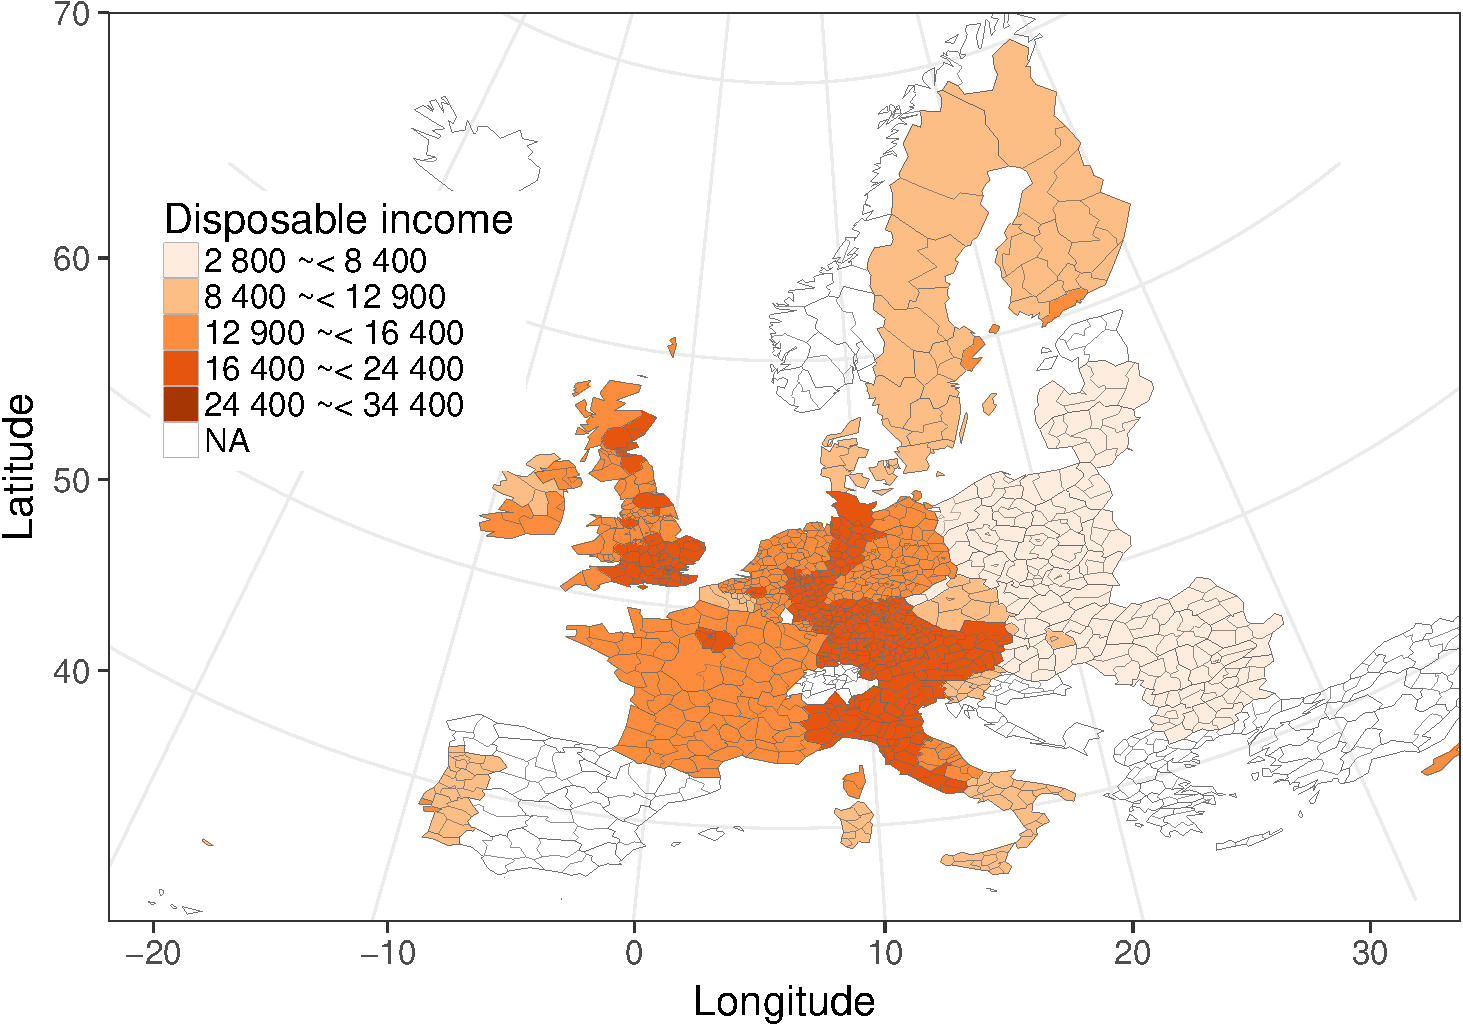
\includegraphics{2015-manu-mapexample-1}
\caption{Disposable income of private households shown on the European map retrieved with the eurostat package and visualized with the aid of additional R extensions.}
\label{fig:mapexample}
\end{center}
\end{figure}




\section{Other functionality}

To facilitate convenient analysis and visualization of standard
European areas, we have included ready-made country code lists for
certain standard areas. To retrieve, for instance, the eurostat
country code list for EFTA as shown in Table~\ref{tab:efta}, use:

\begin{example}
data(efta_countries)
\end{example}

Such country listings are available for EFTA (efta\_countries), Euro
area (ea\_countries), EU (eu\_countries) and EU candidate countries
(candidate\_countries) [MENTION WHICH COUNTRY CODING SYSTEM IS BEING
USED HERE]. These auxiliary data sets facilitate fast selection of
specific country groups. Conversions between different country coding
standards are available with the \CRANpkg{countrycode} R
package \citep{countrycode}.


\begin{table}[ht]
\centering
\begin{tabular}{rll}
\toprule
  \hline
  & code & name \\ 
  \hline
  1 & IS & Iceland \\ 
  2 & LI & Liechtenstein \\ 
  3 & NO & Norway \\ 
  4 & CH & Switzerland \\ 
   \hline
\bottomrule   
\end{tabular}
\label{tab:efta}
\caption{The EFTA country code table as provided by the eurostat R package.}
\end{table}

The downloaded data sets are stored in cache by default to avoid
repeated downloads of identical data sets, helping to speed up the
analysis. Another advantage is that an exact copy of the retrieved
data on the hard disk makes it possible to reproduce the analysis
results even when the source database is updated.


\section{Summary}

The eurostat R package provides convenient tools to access open data
from Eurostat. Integrating automated access to the data sets with
further data analysis and visualization tools provided in other
packages allows a seamless automation of the data analytical workflow
from accessing the raw data to statistical analysis and final
publication. For the full reproducible source code of the figures and
tables of this manuscript, see the package Github
site\footnote{https://github.com/rOpenGov/eurostat/blob/master/vignettes/manuscript.Rmd}. The
reproducible Rmarkdown document provides transparent documentation
with full algorithmic details on how to access, preprocess, analyse,
and report data and analyses, and can be also used to update the
material when new or updated versions of the Eurostat data become
available.

The package provides one set of solutions to automated data retrieval
from independent data repositories, featuring options such as search,
subsetting and cache. Possible future extensions and improvements
include implementation of specific data representation formats to
harmonize the data representation [LINK TO PANEL-SERIES DATA HERE]
across similar data sources and to facilitate subsequent tool
development.

The latest development version of the package can be installed from
Github by following the instructions at the github
site\footnote{https://github.com/rOpenGov/eurostat}. The package
source code can be freely used, modified and distributed under the
BSD-2-clause (modified FreeBSD) license. We welcome issues, bug
reports and other feedback via the development
site\footnote{https://github.com/ropengov/eurostat}.


\section*{Acknowledgements}

We are grateful to Eurostat\footnote{http://ec.europa.eu/eurostat} for
maintaining the open data portal and the
rOpenGov\footnote{https://github.ropengov.io} for supporting 
package development. This work has been partially funded by Academy of
Finland (decision 293316). We also wish to thank Juuso Parkkinen and Joona Lehtomaki for their feedback on this work.


\bibliography{lahti-huovari-kainu-biecek}

\address{Leo Lahti\\
  Department of Mathematics and Statistics\\
  PO Box 20014 University of Turku\\
  Finland\\}
\email{leo.lahti@iki.fi}

\address{Janne Huovari\\
  Affiliation\\
  Address\\
  Country\\}
\email{author2@work}

\address{Markus Kainu\\
  Affiliation\\
  Address\\
  Country\\}
\email{author3@work}

\address{Przemyslaw Biecek\\
  Faculty of Mathematics, Informatics, and Mechanics\\
  University of Warsaw\\
  Banacha 2, 02-097 Warsaw\\
  Poland\\}
\email{P.Biecek@mimuw.edu.pl}

